\documentclass[11pt,a4paper]{article}
\usepackage[utf8]{inputenc}
\usepackage[T1]{fontenc}
\usepackage[english]{babel}
\usepackage{amsmath}
\usepackage{graphicx}
\usepackage{geometry}
\usepackage{hyperref}
\usepackage{float}
\geometry{margin=2.5cm}

\begin{document}

%TITLE PAGE
\begin{titlepage}
    \centering
    \vspace*{2cm}
    
    \Large \textbf{Warsaw University of Technology} \\
    \large Faculty of Power and Aeronautical Engineering \\
    
    \vspace{4cm}
    
    \huge \textbf{Investigation of Stability Limits and Flame Quenching Phenomena of Methane Combustion at High Exhaust Gas Recirculation Rates} \\
    \vspace{0.5cm}
    \Large \textit{1D Kinetic Numerical Analysis Using Cantera Framework}
    
    \vspace{4cm}
    
    \begin{flushleft}
    \large
    \textbf{Author:} Jan Piasecki \\
    \textbf{Student ID:} 333486 \\
    \vspace{0.5cm}
    \textbf{Course:} Computer Methods in Combustion (MKWS) \\
    \textbf{Supervisor:} dr inż. Mateusz Żbikowski \\
    \end{flushleft}
    
    \vfill
    
    \large June 2026
    
\end{titlepage}

%TABLE OF CONTENTS
\pagenumbering{roman}
\tableofcontents
\newpage

%MAIN CONTENT
\pagenumbering{arabic}

\begin{abstract}
This report presents a numerical analysis of the impact of Exhaust Gas Recirculation (EGR) on the propagation and stability of a one-dimensional, laminar methane flame. Utilizing the Cantera software package and the GRI-Mech 3.0 kinetic mechanism, the flame behavior was investigated as a function of the air excess ratio ($\lambda$) and the increasing mass fraction of carbon dioxide in the oxidizer stream. The primary objective was to determine the critical stability limits (flame quenching limits) by applying a physical minimum velocity criterion coupled with an advanced numerical bisection method. The results demonstrate that the addition of an inert gas with high heat capacity significantly narrows the flammability limits of methane, ultimately leading to flame extinction.
\end{abstract}
\fontsize{13}{15.5}\selectfont 
\vspace{1cm}
\section{Introduction}
Exhaust Gas Recirculation (EGR) is a crucial technology employed in modern combustion systems to mitigate nitrogen oxide ($NO_x$) emissions. Although the addition of exhaust gases effectively lowers peak combustion temperatures, excessive dilution leads to kinetic instability and, eventually, to the break-off of the flame front (flame quenching). Unlike zero-dimensional (0D) analyses focusing solely on autoignition delay, this study utilizes a one-dimensional freely propagating flame model (1D FreeFlame). This approach allows for direct observation of the physical suppression of burning velocity leading up to complete mixture extinction.

\vspace{1cm}
\section{Literature Review}
Understanding the theoretical limits of EGR dilution is paramount for modern low-emission burner design. It should be clarified that in this study, for simulation purposes, the EGR dilution is implemented as a molar $CO_2$ fraction to strictly control the reactant pool kinetics. This methodology aligns with standard kinetic testing protocols for isolating thermal dilution effects. Experimental results from broader combustion literature regarding $CH_4$/air/$CO_2$ mixtures suggest that complete extinction of a stoichiometric laminar flame typically occurs when the $CO_2$ mole fraction reaches critical limits of approximately $24-26\%$. As will be demonstrated, the numerical extinction limit computed in this study ($28.44\%$) exhibits reasonable agreement with these documented physical phenomena. The observed overprediction of the dilution tolerance is an expected limitation of the model, primarily attributable to the ideal adiabatic assumption and the lack of radiative heat loss considerations in the simulated 1D domain.
\newpage
\section{Methodology and Numerical Model}

\subsection{Simulation Setup}
The calculations were performed using Python and the Cantera thermochemical toolkit. The GRI-Mech 3.0 reaction mechanism (comprising 53 species and 325 elementary reactions), optimized for natural gas combustion, was utilized. The simulations were conducted at atmospheric pressure ($P = 1 \text{ atm}$) and an initial unburned gas temperature of $T_0 = 300 \text{ K}$. The air excess ratio was varied within six evenly spaced points in the range of $\lambda \in [0.8, 1.3]$.
\vspace{1cm}
\subsection{Governing Equations and Physical Limits}
The one-dimensional freely propagating flame is governed by the conservation equations for mass, species, and energy. For a steady, isobaric, 1D flame, the energy conservation equation solved by Cantera is:

\begin{equation}
    \rho c_p \frac{dT}{dx} = \frac{d}{dx}\left( k \frac{dT}{dx} \right) - \sum_{k=1}^{K} \dot{\omega}_k h_k M_k - \rho \sum_{k=1}^{K} c_{p,k} Y_k V_k \frac{dT}{dx}
\end{equation}

Where $\rho$ is the density, $c_p$ is the specific heat capacity at constant pressure, $T$ is the temperature, $x$ is the spatial coordinate, $k$ is the thermal conductivity, and $\dot{\omega}_k$ is the molar production rate of species $k$.

\textbf{Physical Extinction Criterion:} The flame is considered extinguished if the computed laminar burning velocity ($S_L$) drops below a critical threshold of $3.5 \text{ cm/s}$. While this value is an engineering assumption rather than a fundamental derived physical constant, it serves as a robust practical criterion to represent realistic extinction limits where conductive and radiative heat losses dominate over chemical heat release.
\vspace{1cm}
\subsection{Advanced Numerical Quenching Detection}
To accurately determine the exact quenching boundary without being constrained by a coarse simulation step grid, a numerical \textbf{bisection method} coupled with a \textbf{warm-start} solver configuration was implemented. Once a coarse quench is detected, the algorithm iteratively halves the interval between the last known stable EGR value and the failed EGR value. During each bisection step, the solver is initialized using the spatial array data from the previous stable flame (\textit{warm-starting}). This approach not only prevents premature solver failure due to stiffness in lean mixtures but also allows for finding the physical limit ($S_L < 3.5 \text{ cm/s}$) with an exceptional tolerance of $0.2\%$.
\newpage
\section{Results and Discussion}

\subsection{Suppression of Laminar Burning Velocity}
The numerical results demonstrate a non-linear, monotonic decrease in laminar burning velocity ($S_L$) with increasing EGR rates across all investigated equivalence ratios. At stoichiometric conditions ($\lambda = 1.0$), pure methane-air combustion yields a baseline propagation speed of $38.21 \text{ cm/s}$. The introduction of $15\% \ CO_2$ reduces this velocity to $12.93 \text{ cm/s}$. 

Two coupled physical mechanisms govern this severe suppression of flame propagation. Firstly, the \textbf{dilution effect}: the addition of inert $CO_2$ molecules decreases the volumetric concentration of reactive species ($CH_4$ and $O_2$), directly reducing the frequency of effective molecular collisions. Secondly, the \textbf{thermal sink effect}: $CO_2$ possesses a significantly higher molar heat capacity than diatomic nitrogen ($N_2$). It absorbs a substantial portion of the exothermic heat released in the reaction zone without contributing to the chemical pathways, thereby retarding the spatial advancement of the flame front.
\vspace{1cm}
\begin{figure}[H]
    \centering
    
    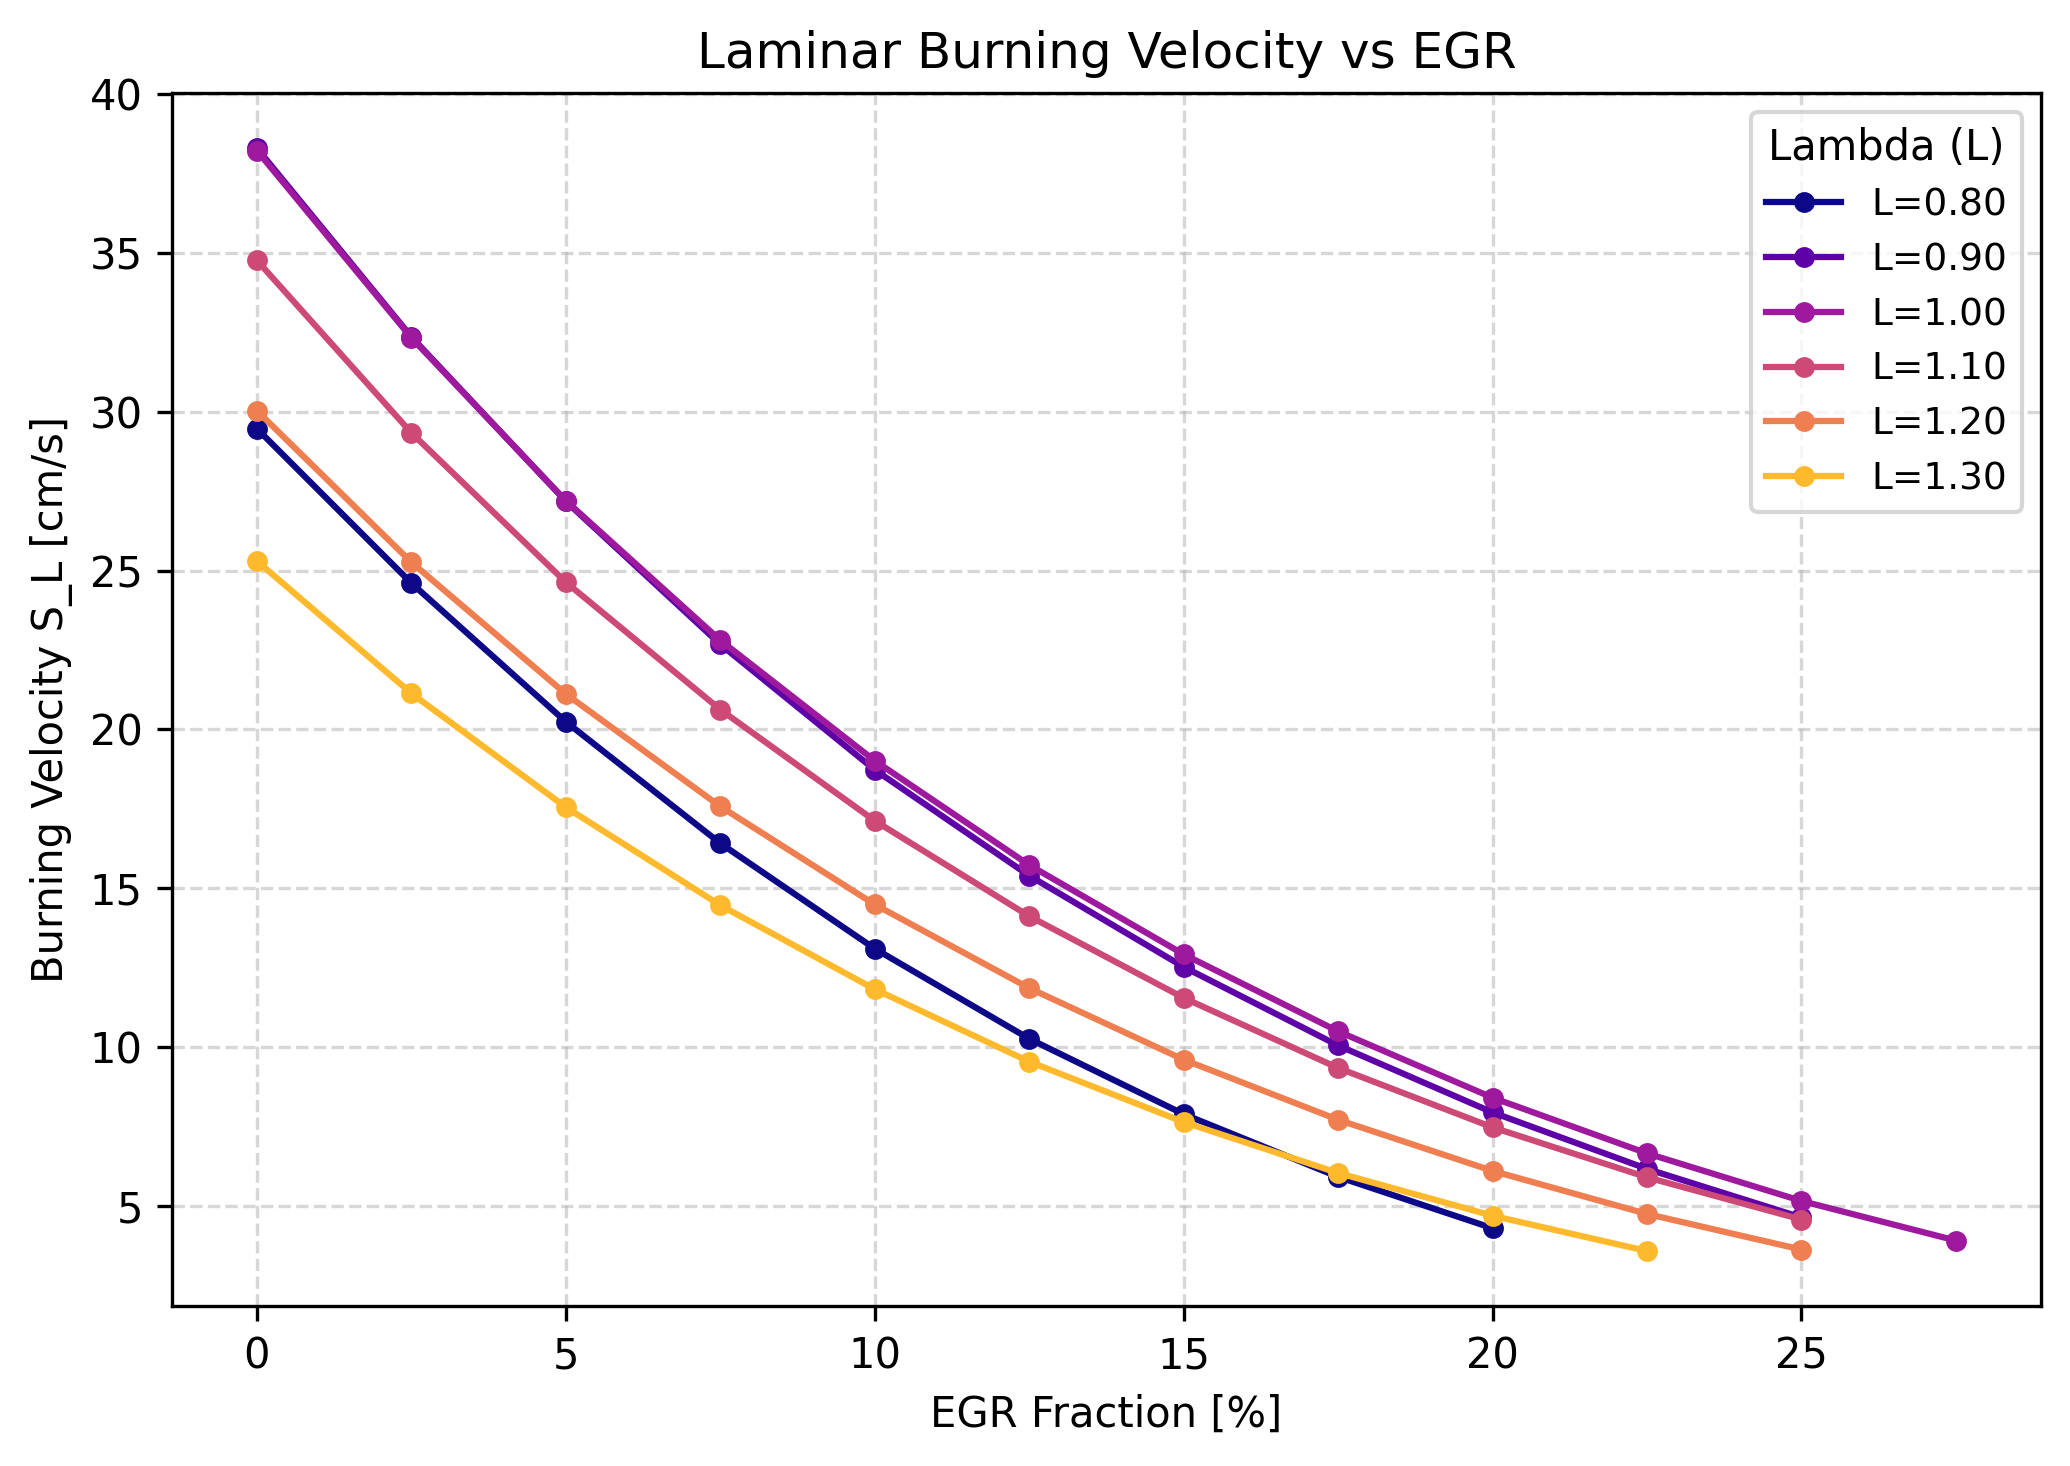
\includegraphics[width=0.8\textwidth]{Wykres_1_Predkosc.png}
    \caption{Laminar burning velocity ($S_L$) as a function of $CO_2$ dilution (EGR fraction).}
    \label{fig:velocity}
\end{figure}

\newpage
\subsection{Reduction of Peak Flame Temperature}
The thermal state of the reaction zone fundamentally drives the kinematic suppression of the flame. As illustrated in Figure \ref{fig:temperature}, each additional percent of $CO_2$ induces a nearly linear, proportional decrease in the maximum adiabatic flame temperature. For instance, at $\lambda = 1.0$, the baseline temperature of $2228.9 \text{ K}$ drops consistently down to the quenching limit near $1668 \text{ K}$.

According to Arrhenius kinetics, the rates of elementary chemical reactions exhibit an exponential dependence on temperature. Therefore, the observed linear temperature reduction translates into an exponential deceleration of the primary chain-branching reactions (such as $H + O_2 \rightleftharpoons OH + O$). The resulting depletion of the radical pool deprives the flame of the chemical energy required to overcome conductive and radiative heat losses, ultimately dictating the physical quenching boundaries.
\vspace{1cm}
\begin{figure}[H]
    \centering
    
    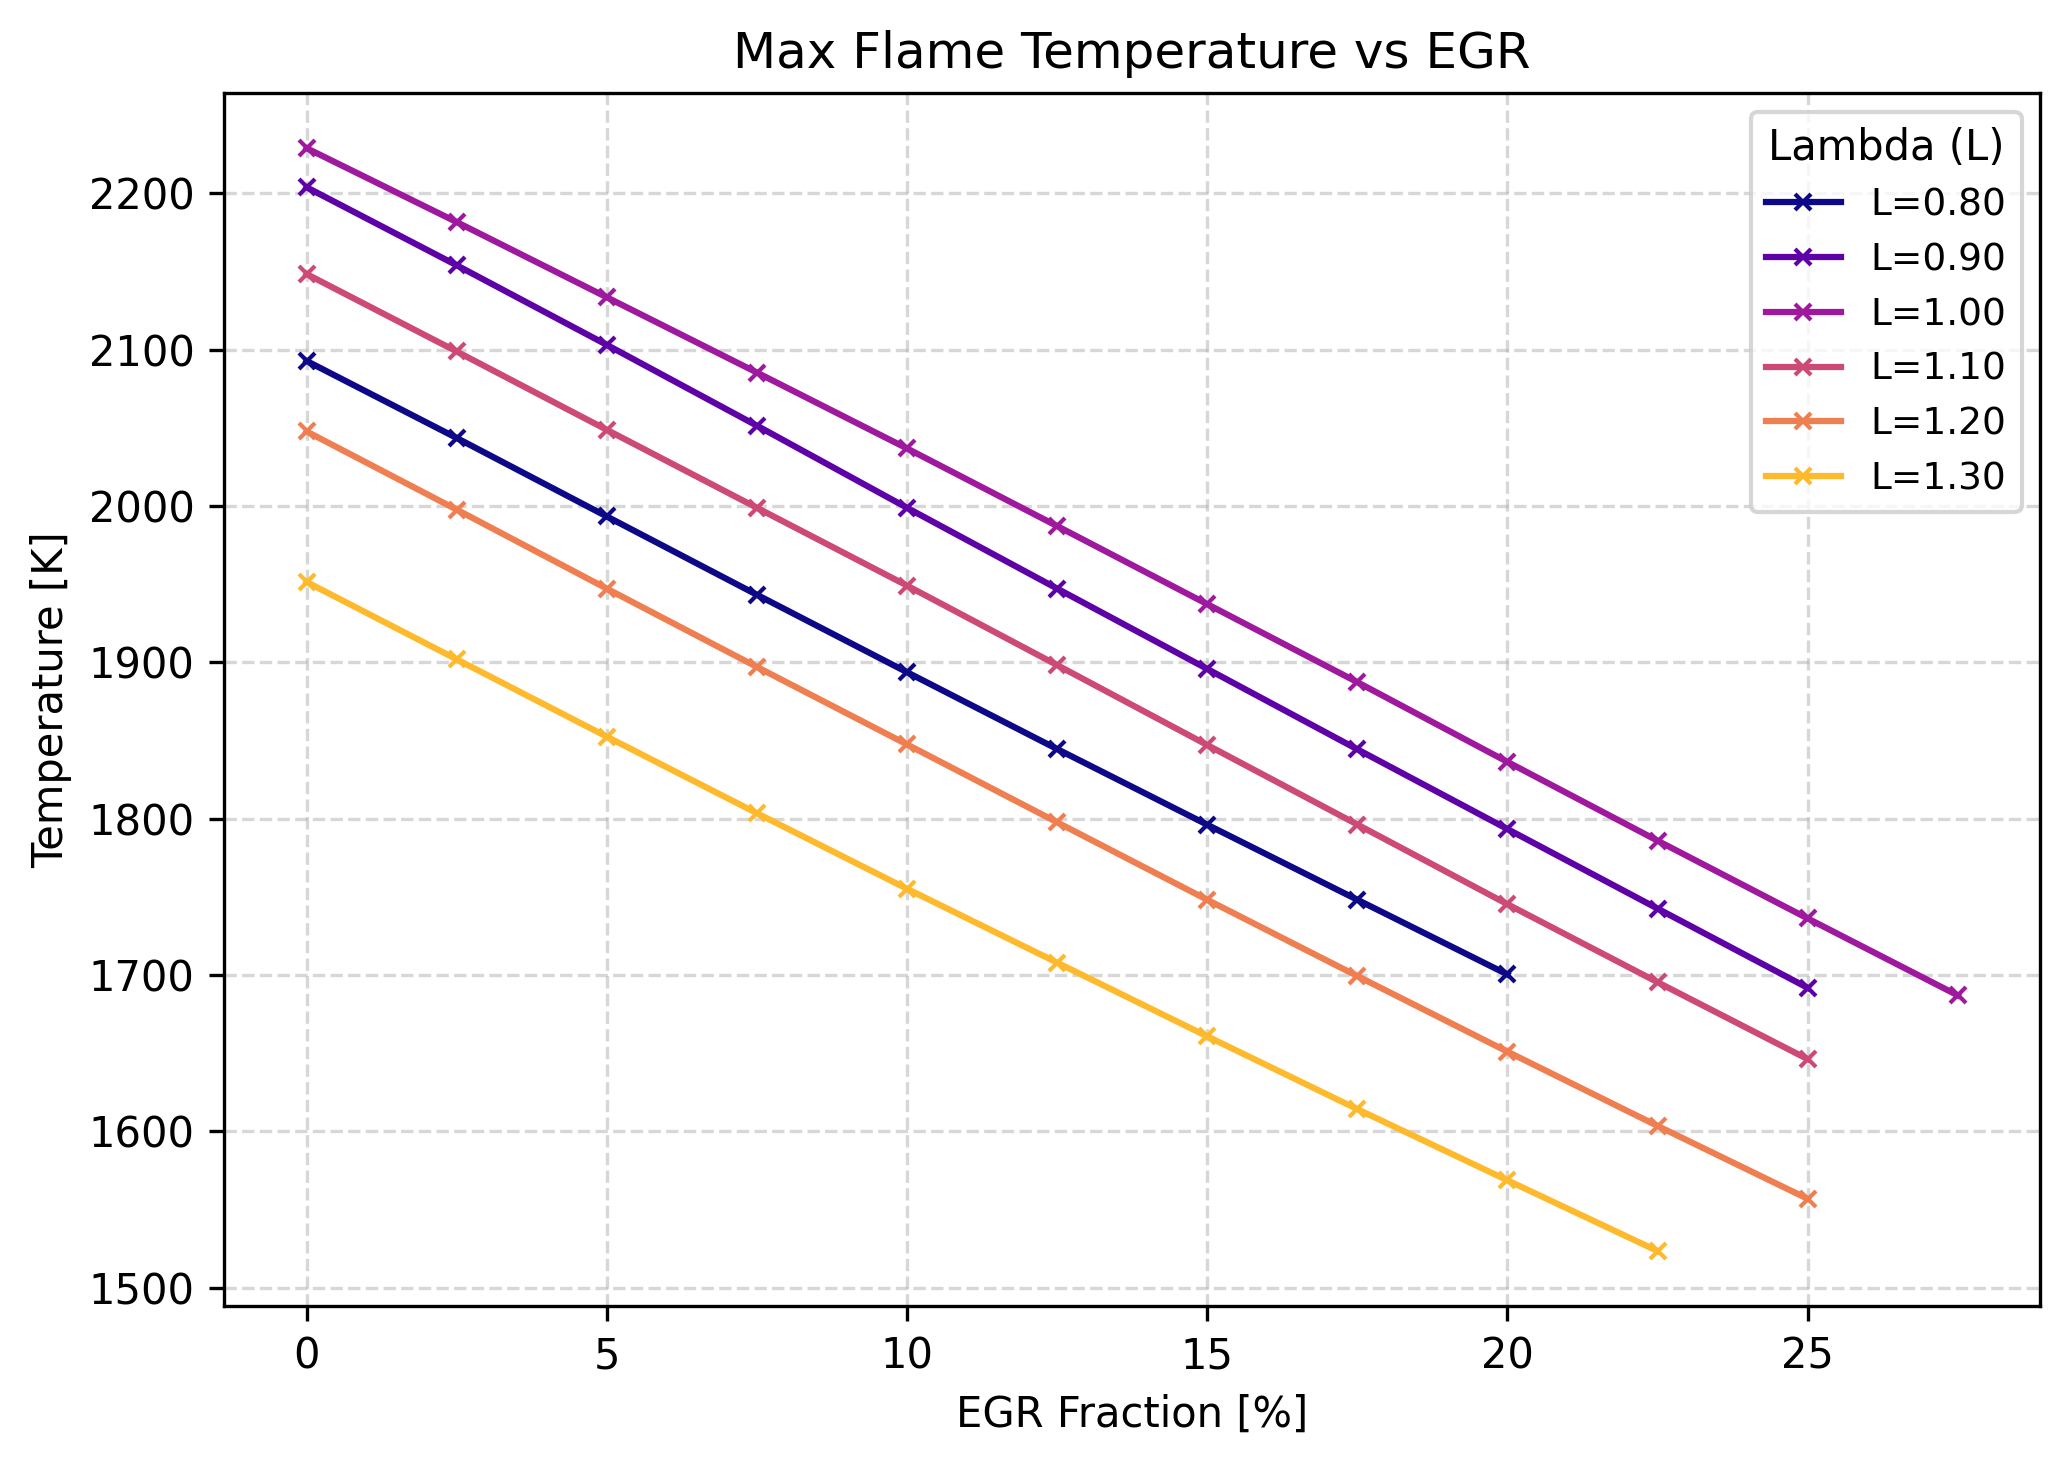
\includegraphics[width=0.8\textwidth]{Wykres_3_Temperatura.png}
    \caption{Maximum adiabatic flame temperature reduction driven by increasing EGR fraction.}
    \label{fig:temperature}
\end{figure}

\newpage
\subsection{Stability Limits Map (Quenching Curve)}
The implementation of the bisection method yielded a highly precise Stability Limits Map. The boundary forms a characteristic arch-shaped profile. The simulation indicates that maximum EGR tolerance occurs near stoichiometry (between $\lambda = 1.0$ and $1.1$), peaking at approximately $28.44\% \ CO_2$ dilution before reaching the $3.5 \text{ cm/s}$ velocity threshold. 

The refined data proves that at both the rich ($\lambda = 0.8$) and lean ($\lambda = 1.3$) boundaries, the physical quenching limits show comparable magnitudes, occurring at values of $21.56\%$ and $22.66\% \ CO_2$, respectively. However, the arch is distinctly asymmetric: the EGR tolerance drops much more steeply on the fuel-rich side ($\lambda < 1.0$) compared to the more gradual, elongated decline observed on the fuel-lean side. This physical behavior arises because excess fuel on the rich side competes differently with the thermal dilution of $CO_2$ than excess air does on the lean side, directly impacting radical pool availability and reaction rates.
\vspace{1cm}
\begin{figure}[H]
    \centering
  
    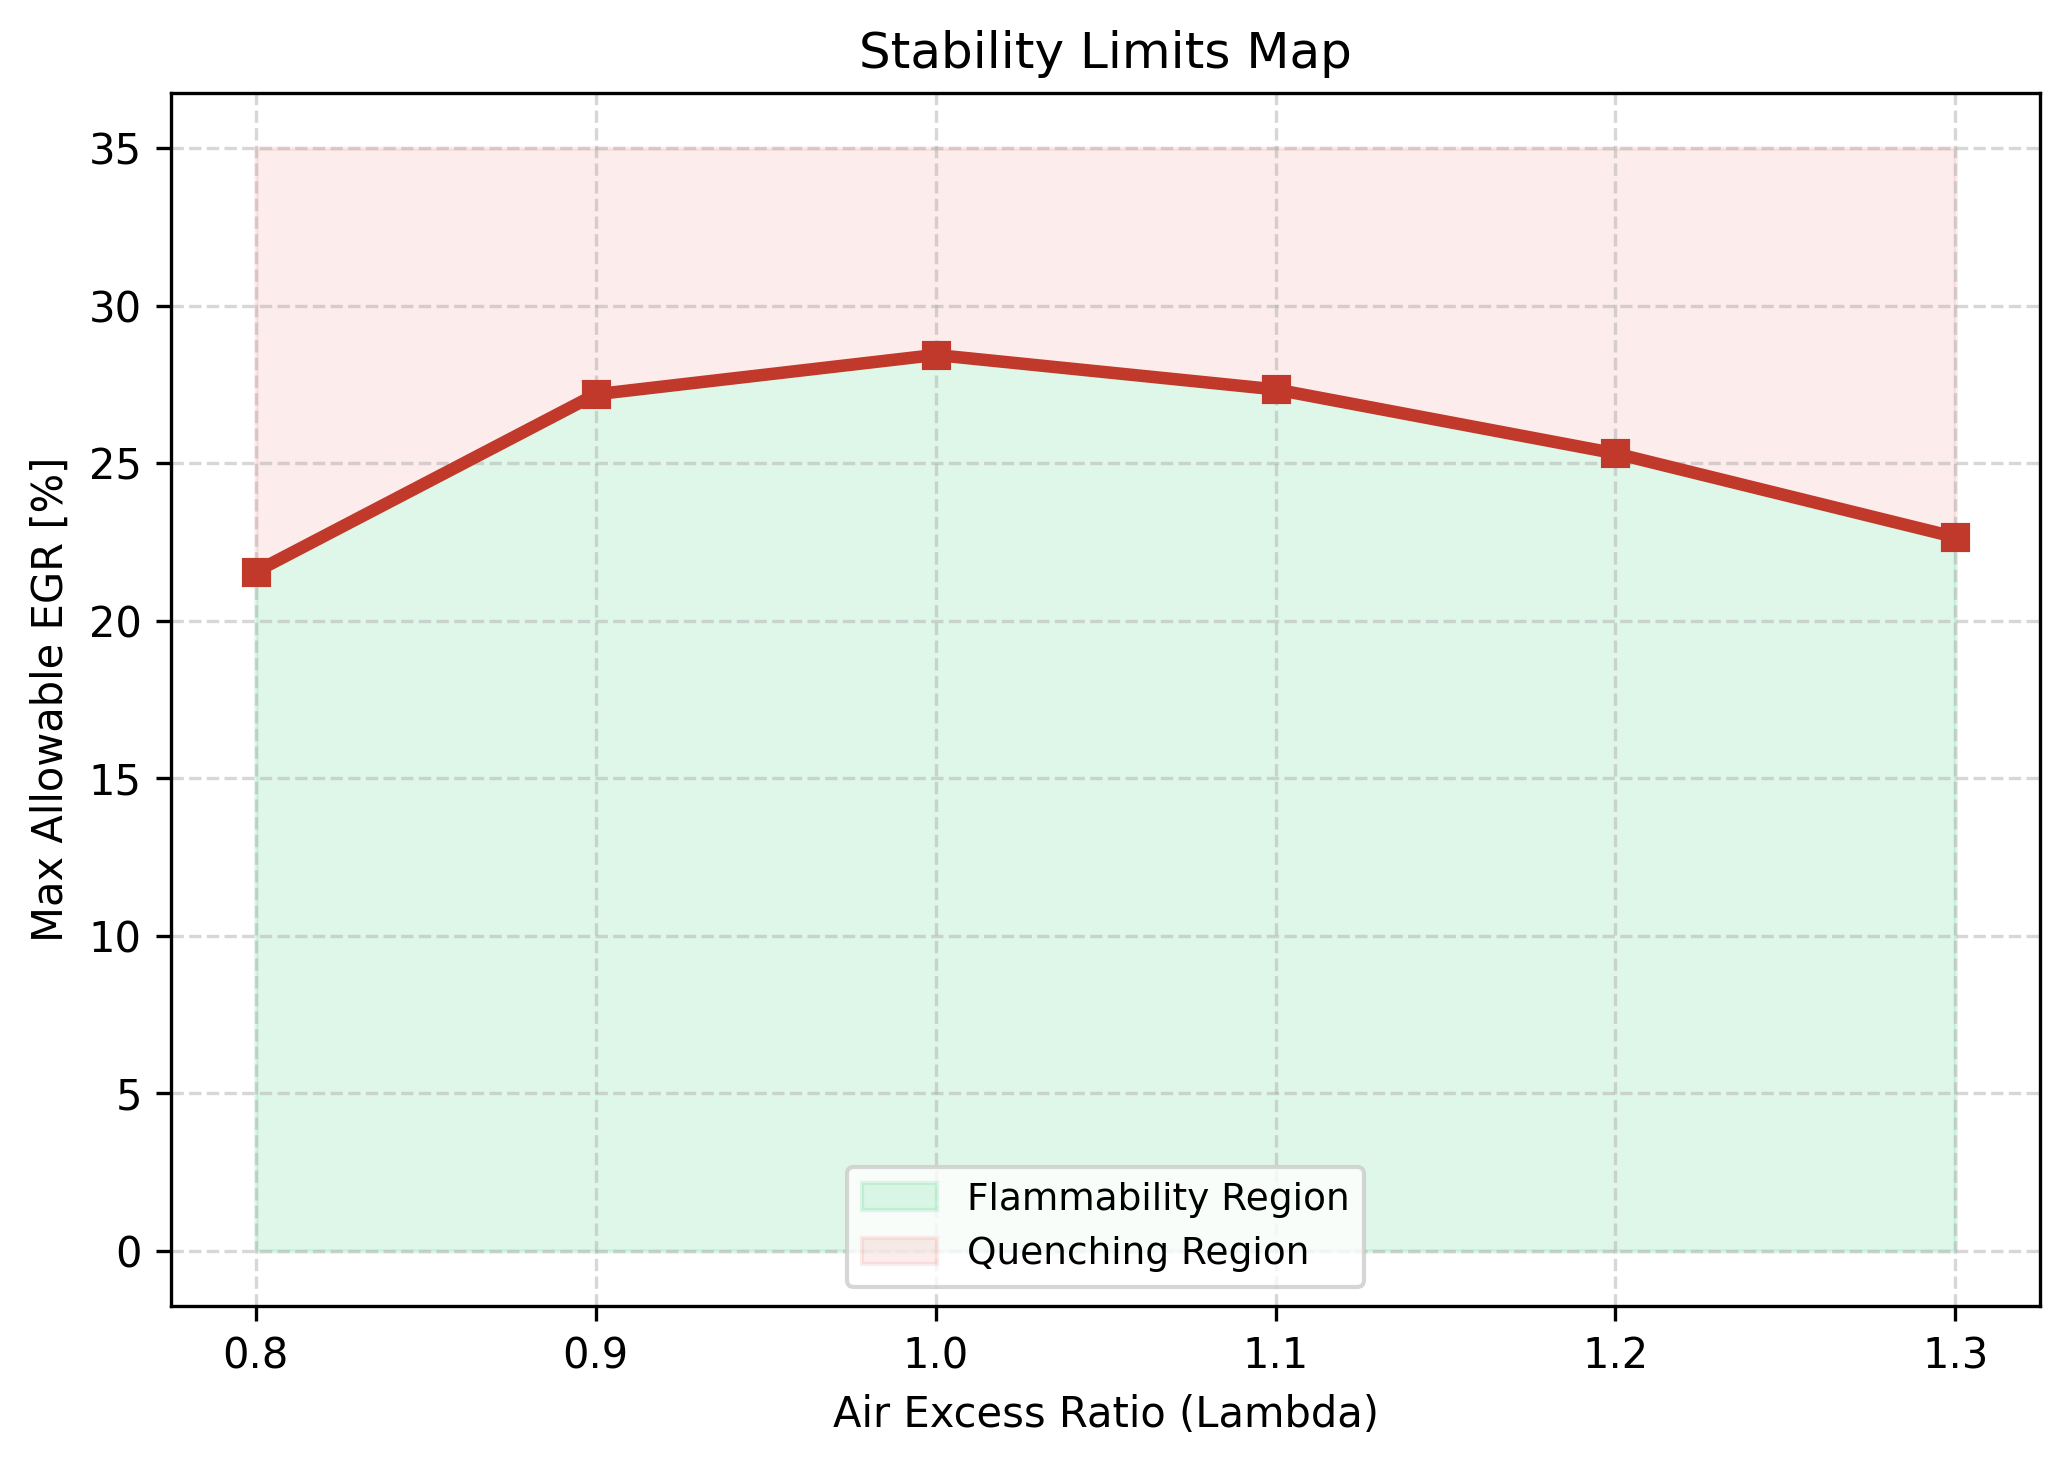
\includegraphics[width=0.8\textwidth]{Wykres_2_Mapa.png}
    \caption{Stability Limits Map illustrating the precise maximum allowable EGR fraction.}
    \label{fig:stability_map}
\end{figure}
\newpage
\section{Conclusions}
\begin{enumerate}
    \item Exhaust Gas Recirculation systems operating with high $CO_2$ mass fractions drastically alter the kinetics and spatial structure of a 1D flame, retarding its propagation velocity primarily due to the increased thermal capacity of the unburned charge.
    \item The introduction of the $3.5 \text{ cm/s}$ engineering flammability criterion successfully replicates realistic flame quenching, confirming that maximum EGR tolerance (up to $28.44\%$) occurs near stoichiometric conditions ($\lambda = 1.0$ to $1.1$).
    \item The stability map reveals a physically asymmetric response to mixture leaning and enriching. The flame's tolerance to $CO_2$ dilution drops more precipitously under fuel-rich conditions compared to fuel-lean conditions, highlighting the complex coupling between reactant availability and the fundamental quenching velocity threshold.
\end{enumerate}
\vspace{1cm}
\begin{thebibliography}{9}
\bibitem{turns}
Stephen R. Turns,
\textit{An Introduction to Combustion: Concepts and Applications},
McGraw-Hill Education, 3rd Edition, 2011.

\bibitem{glassman}
Irvin Glassman, Richard A. Yetter, and Nick G. Glumac,
\textit{Combustion},
Academic Press, 5th Edition, 2014.

\bibitem{cantera}
D. G. Goodwin, R. L. Speth, H. K. Moffat, and B. W. Weber,
\textit{Cantera: An Object-oriented Software Toolkit for Chemical Kinetics, Thermodynamics, and Transport Processes}, Version 3.0.0, 2023.
\end{thebibliography}

\end{document}